\chapter{Преглед на съществуващите системи}

Писането на тази секция представлява особена трудност, тъй като реално
погледнато не същестува еквивалент на системата изложена в настоящата
дипломна работа. Същестуват много речникови приложения, като някои от
тях имат и изпитен модул, но обикновено тук свършват техните
възможности. 

Може би ще прозвучи нескромно, но просто не същестува двуслойна
система(десктоп клиент + уеб приложение), десктоп клиентът, за която
на всичкото отгоре да е портативен между операционните системи и да
позволява на потребителите активно да допринасят за разширяването на
речниковия му фонд. В една система за езиково обучение именно той
представлява най-ценния ресурс, поради простата причина, че каквито и
модули да включва в себе си системата те ще имат нужда от някакъв
речников фонд.

Освен това Spellbook е проект с отворен код и е напълно безплатен за
потребителите. Фирми като KoralSoft и Gaberoff предлагат някои
по-пълни обучителни системи, но те са доста скъпи.

Преди да преминем към конкретните сравнения искам да отбележа и факта,
че за разлика от много проекти Spellbook поставя огромен фокус върху
комуникацията с крайните потребители, отвореният процес на разработка
и използването на модерни технологии. Голяма част от речниковите и
обучителни системи, които съществуват в момента нямат официални
страници(или разполагат с някаква пародия на страница), нямат грам
прозрачност в разработката си и потребителите са в пълно неведение
кога какво се случва(и дали въобще нещо се случва), а участието им в
проекта обикновено се свежда просто до използването му. Spellbook не е
такъв проект - огромна част от интересните му възможности не са се
родили от ограничената фантазия на неговия автор, а са плод на идеи и
желания на неговите потребители. В пощенският списък на приложението
се водят често интересни дискусии, а също така и в неговата система за
следене на грешки.

След тази кратка овертюра ще преминем към историята родила проекта и
сравнение с основните му конкуренти.
\section{Роден от необходимост}

Ще си позволя да напиша следващите няколко реда в по-неформален
маниер, тъй като Spellbook се роди изцяло от моите лични нужди и се
разви отвъд моите първоначални планове за да стигне до комплексната
система за езиково обучение, която представям в тази дипломна работа.

В последните 7 години аз екслузивно използвам GNU/Linux операционни
системи(най-вече Arch Linux и Fedora). Въпреки, че познанията ми по
английски се считат за отлични, дори на мен от време на време ми се
налага да използвам речниково приложение. Винаги съм предпочитал
десктоп приложенията за тази цел, тъй като те работят постоянно във
фона на операционната ми система, интегрират се със системния
клипборд(мога да превеждам дума само като я копирам там) и като цяло
са по-удобни за работа от набиращите огромна популярно уеб
приложения. Освен това в едно десктоп приложение все още е възможно да
бъде разработен по-гъвкав, красив и функционален потребителски
интерфейс. 

В годините, през които бях потребител на Windows имах голям избор от
речникови програми на разположение и основно използвах чудесният
речник SA Dictionary, разработен от Стефан Ангелов. За него ще говоря
малко повече в следващата секция. Когато мигрирах към GNU/Linux,
обаче, се оказа, че далеч не същестува такъв избор. Всъщност има едно
единствено речниково приложение за GNU/Linux за GNOME(графичната
среда, която използвам аз), което включва в себе си
двупосочен(или като аз го наричам комплементарен) речник, а именно
gbgoffice, част от проекта BG Office. gbgoffice е написан на C++ през
далечната вече 2004 година, като послената му версия е от 2006
година. След като приложението ми служи вярно няколко години в един
момент се оказа, че то просто не се компилира вече с актуалните версии
на g++ компилатора и gtkmm библиотеката. Тъй като приложението е с
отворен код и аз съм работил дълго време като C програмист за мен
нямаше да представлява особен проблем да поправя проблемния код и да
продължа да използвам gbgoffice, но мисълта че ползвам неподдържан
софтуер определено щеше да ме дразни, а аз никога не съм бил по
полoвинчатите решение на проблемите. 

По това време вече бях приключил с кариерата си на C/C++ програмист и
се бях преориентирал към Java. В последните години бях придобил
приличен опит в разработката на графични потребителски интерфейси на
Swing и SWT и затова си казах - "`Абе колко му е човек да напише един
прост речник на Java и Swing и да си го ползва навеки?"'. Така нямаше
да съм вече зависим от прищевките на някой неоткриваем разработчик и
щях да имам софтуера, от който се нуждая. Когато започнах да работя по
проектчето в свободното си време преди около 9 месеца то си нямаше име
и се казваше просто dictionary(речник на английски). В първата му
версия нямаше почти никаква функционалност - просто въвеждаш дума и
виждаш превода и. За речникова база бях използвал речниците от
gbgoffice, които декодирах от двоичния им формат и въведох в
релационна база данни. Реших, че може би и други хора имат моя проблем
с липсващите речникови системи под GNU/Linux и споделих в една тема
във форумите на популярният портален сайт за Линукс потребители
"`Линукс за българи"', че работя по малък английско-български речник,
който по принцип е платформено независим, но вероятно ще представлява
най-голям интерес за Линукс потребителите с оглед на липсата на
алтернативи за тях. Оказа се, че доста хора са заинтересовани от
разработката ми и затова веднага направих един малко по-прегледен сайт
в Google Code и измислих име на проекта(защото никой уважаващ себе си
проект не може да се казва просто dictionary). Щеше ми се името да не
бъде пряко свързано с речници, за да мога евентуално да разширя
фунционалността на приложението(както и се случи в последствие). Спрях
се на името \textbf{Spellbook}, тъй като ми хареса играта да думи в
него. Думата spellbook принципно значи \emph{"`книга с магии"'}, но думите
spell и book по отделно мога да се тълкуват като \emph{"`сричам"'} и
\emph{"`учебник"'} - \emph{учебник за сричане} - хубаво име за една система за
езиково обучение. 

Така на 25.10.2009 се роди версия 0.1 на Spellbook. Тя бе ознаменувана
само с кратък анонс в "`Линукс за българи"'. Текстът му беше следния:

\emph{Spellbook Dictionary е платформено независим речник(понастоящем
  двупосочен английско-български), написан на Java. Проекта се стреми
  към простота на ползване и възможност за лесно разширяемост в
  бъдеще, както и да консолидира усилията за създаване на стандартен
  свободен речник с богата база данни. 
Благодарности на проекта БГ Офис, чиято база използваме в Spellbook
като отправна точка.}

В рамките на седмица от анонса Spellbook 0.1 беше изтеглен от над 100
души. В рамките на първия месец - от над 300! Това сериозно
надвишаваше очакванията ми, тъй като "`Линукс за българи"' не е
посещавам от много хора. Един от най-учудващите моменти за мен беше,
когато брат ми един дем ми разказа как негов колега го попитал дали
има роднинска връзка с автора на Spellbook Божидар Бацов. Явно имах
потребители на най-неочакваните места! Този първоначален успех ме
мотивира да запретна ръкавите и направя една много по-мощна система,
далеч отвъд възможностите на прост речник. 

По същото време водех и свободно избираем курс по програмиране на Java
в ТУ-София и имах нужда от някакви практически упражнения за
студентите ми там. Беше ми омръзнало да им давам само дребни
синтетични задачки за упражнения, исках да усетят атмосферата на
работата по инстински проект и да придобият ценен практически опит за
работата в екип и за екосистемата на професионалните проекти - работа
с хранилище на код, система за следене на грешки, пощенски списъци,
писане на тестове и т.н. Исках и да ги предизвикам да мислят - затова
ги подканих да дадат идеи за модули за приложението. Модулите за
проверка на правописа и учене на думи са резултат от предложения на
тези студенти. На най-дейните от тях дадох права да работят по някои
по-малки задачки в проекта - отзивите от тяхна страна бяха много
ласкави. Възможността да работят по истински проект им помогнала много
за да впрегнат научените неща в университета и моя курс досега.

Благодарение на потока на идеи ентусиазмът ми беше допълнително
увеличен и следващите няколко месеца пуснах две нови версии на
Spellbook - 0.2(31.12.2009) и 0.3(12.05.2010), които разшириха много
първоначалните му възможности и подобриха значително реализацията
му. Надявам се в близките няколко месеца да достигнем първата версия
включваща абсолютно всичко(feature complete), което желая да има в
системата на този етап - знаменателната версия 1.0. Още повече се
надявам системата да продължи да расте и да се развива отвъд версия 1.0.

Моята визия за Spellbook е това да е една система развивана от
потребителите, подобно на приложения като \emph{Wikipedia} и
\emph{YouTube}, чиито огромен успех се дължи само и единствено на
много потребители, които допринасят за разширавянето на съдържанието
там. Ако Spellbook има 1000 потребители и 100 от тях допринасят по 10
думи всеки ден - това са над 350 хиляди нови думи годишно! По-голям
речников фонд в комбинация с уникални възможности би разширил още
потребителската база. Това в момента е само теория, разбира
се. Времето ще покаже доколко е вярна тя. Във всеки случай от самото
начало беше част идеята приложението да има уеб и десктоп версия. В
ерата на интернет технологиите е несериозно да се пренебрегва този
паразен сегмент. За нещастие, аз бях твърде зает да и отделя време, но
пък тук се намеси моя добър приятел и колега инж. Иван Хантов, който
се съгласи да разработи уеб приложението, което също ще бъде
представено като дипломна работа. Според мен симбиозата между десктоп
и уеб технологиите е ключова за успеха на повечето продукти.

Това, разбира се, не е краят на развитието откъм платформи, на които
може да работи приложението. В момента мобилните устройства като ipod,
ipad, iphone и google android телефоните доминират пазара и е напълно
възможно някой ден да видим версия на Spellbook за някои от тях.
\section{Преглед на конкурентните системи}
Конкурентните системи могат най-общо да бъдат разделени на три групи -
десктоп приложения, уеб приложения и комбинирани приложения(десктоп +
уеб). Приложения в третата категория няма(поне доколкото аз съм
запознат), което прави Spellbook уникален заради неговия самостоятелен
Swing клиент и възможността му да комуникира с уеб версията на
приложението разработена като отделна дипломна работа от колегата Иван
Хантов. 

В сравнението няма да включа компютърните езикови самоучители, тъй
като тяхното разработване изисква много повече ресурси отколкото могат
да бъдат отделени от един човек, работещ по проект в свободното си
време. На практика всички компютърни самоучители са контролирани от
фирми. 

\subsection{Конкурентни десктоп системи}
В секцията "`Речници"' на популярният сайт download.bg има записани
цели 138 приложения. На първо място с огромен аванс пред конкуренцията
по брой изтегляния е \emph{SA Dictionary}. В списъка огромният брой
приложения са просто двупосочни английско-български речници, макар, че
има и някои интересни изключения.
\begin{itemize}
  \item \textbf{SA Dictionary}

    SA Dictionary вече дълги години е най-известната речникова
    програма в България. Основните и плюсове са много богатия
    двупосочен английско-български речник(отскоро е включен и френски
    речник), приличният изпитен модул и малкото ресурси, които
    използва. Авторът на SA Dictionary го описва по следния начин -
    \emph{Най-популярният речник в България за превод на думи от
      английски на български и обратно. Тази версия включва 2 речника
      - англо-български (ок. 120 000 думи) и българо-английски
      (ок. 100 000 думи). Освен това, имате възможност да проверите
      бързодействието на компютъра си с функцията benchmark, измерваща
      броя преведени думи за секунда. Добавени са англо-български
      речник с компютърни термини (ок. 500 термина), български
      синонимен речник (25 000 думи) и френски речник (25 000 думи).}
    
    \begin{figure}[htbp]
      \caption{SA Dictionary}
      \centering
      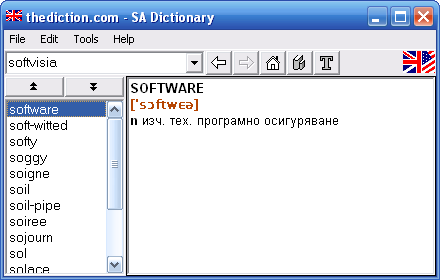
\includegraphics[width=90mm, height=70mm]{images/sa-dictionary.png}
    \end{figure}

    Основните и минуси са хаотичният цикъл на разработката(никога не
    се знае кога точно ще излезе нова версия, в последните години
    текущата версия обикновено винаги има Beta в името си), липсата на
    допълнителни функции, скромният сайт, трудната комуникация с
    автора, и фактът, че приложението макар и да е безплатно не е
    свободен софтуер. Аз самият се опитах да установя неуспешно връзка
    с неговия автор за да го попитам какви са условията му за
    споделяне на речниковата му база данни. Освен всичко гореизброено
    софтуерът работи само под операционната система Windows.

    Когато теглим чертата на накрая SA Dictionary е просто един
    речник, който просто някакси успява да стане доста популярен,
    най-вероятно заради факта, че беше може би първият такъв продукт и
    хората просто са свикнали с него и не се оглеждат за алтернативни
    приложения. Това е често срещано явление в ИТ сферата и причината
    много некачествен софтуер все още да се използва(справка Internet
    Explorer 6 - дори Microsoft се отрекоха от него, но много хора
    продължават да го използват и това създава глобални проблеми).

  \item \textbf{EuroDict}

    Комерсиален речников софтуер, който предлага няколко безплатни
    речника и няколко платени. Софтуерът работи само под Windows и не
    притежава никакви друго допълнителни възможности. Голямото
    предимство на EuroDict е богатата му речникова база - той предлага
    двупосочни немско-български, испано-български, италиано-български,
    френско-български и други речници. В момента една от задачите пред
    Spellbook е да разшири базовия си речников фонд - една от идеите,
    по които се работи е да се изготви конвертор за свободните речници
    от проектът Babylon, което би дало на Spellbook моментално достъп
    до стотици речници.

    Програмата работи само под операционната система Windows.

  \item \textbf{Interlex}

    Interlex е безплатна програма, която освен, че ще ви помогне да
    научите по-лесно чужд език, ще играе и роля на тетрадка
    речник. Принципът й на действие е следния: според авторите за
    по-удобно и успешно запаметяване на думите е необходимо първо да
    се пишат, след което да се четат (като при четенето те вече са
    подредени по азбучен ред). Можете да попълвате думи от всякакви
    езици, заедно с техния превод и транскрипция в Interlex. А след
    това програмата ги извежда като списък. Имате възможност да
    въвеждате отделните думи под различни (каквито ви хрумнат)
    категории. По принцип, продуктът си разполага със завидно богата
    база за учене. Има обемисти речници в превод от руски, испански,
    френски, немски, италиански, гръцки, унгарски норвежки, полски,
    португалски, румънски, шведски, турски, холандски, финландски на
    английски език. Винаги можете да добавяте/премахвате думи и изрази
    от готови речници; да редактирате; да вмъквате коментари,
    обозначения за част от речта (съществително, прилагателно,
    глагол).

    Interlex е безплатна програма, но не е свободен софтуер. Тя по
    същество е надстройка над съществуващата функционалност за учене
    на думи в Spellbook. Планът в Spellbook е, разбира се, секцията за
    учене да думи също да бъде разширена с изрази, а и с граматически
    упражнения. Освен това за разлика от Spellbook Interlex не е
    предназначен специално за родните потребители.

    Програмата работи само под операционната система Windows.

  \item \textbf{AEnglish Dictionary}

    AEnglish Dictionary ви предлага aнглийско-български речник с над
    250 000 думи и фрази, "`превод на живо"' от Internet Explorer,
    Word, Wordpad, Notepad и др., търсене на изрази и думи, създаване
    на собствени листове с думи и получаване на файл с превод за всяка
    от тях, лист с всички наскоро прегледани думи (история), опростен
    интерфейс с възможност за зареждане на теми (скинове), специална
    система от shortcut-и за бърза и лесна работа с речника,
    възможност за заключване на превода и множество опции. По-голямата
    част от това описание е копирана от страницата на проекта. Там той
    е обявен за конкурент на SA Dictionary, но видимо е изоставен -
    последната му версия е от 2003 година.

    Проектът е неподдържан, не предлага нищо повече от един
    двупосочен английско-български речник и макар, че е безплатен, не
    е свободен софтуер - ако беше такъв някой можеше да продължи
    разработката му след видимото оттегляне на оригиналния
    автор. Всички негови възможности освен импортирането на думи от
    файл са достъпни в Spellbook, а липсващата възможност е много
    лесна за реализиране.

    Това е и поредната програма, която работи само под Windows.

  \item \textbf{gbgoffice}

    gbgoffice е GTK2 (gtkmm) версия на популярния пакет
    kbgoffice. Gbgoffice се разработва под Arch Linux и е тестван за
    правилна работа под Slackware, Debian, Fedora, Mandrake, Gentoo и
    FreeBSD. Включва всички речници на проекта BG Office, а именно
    двупосочен английско-български речник, речник на компютърните
    термини, политехнически английско-български речник, синонимен
    речник и речник на северозападния диалект. Общо взето на този етап
    това са и речниците на Spellbook, тъй като той използва за база
    същите речници от проекта BG Office. Както изтъкнах по-горе,
    обаче, в момента активно се работи за включване на двупосочни
    речници за основните езици. 

    \begin{figure}[htbp]
      \caption{gbgoffice}
      \centering
      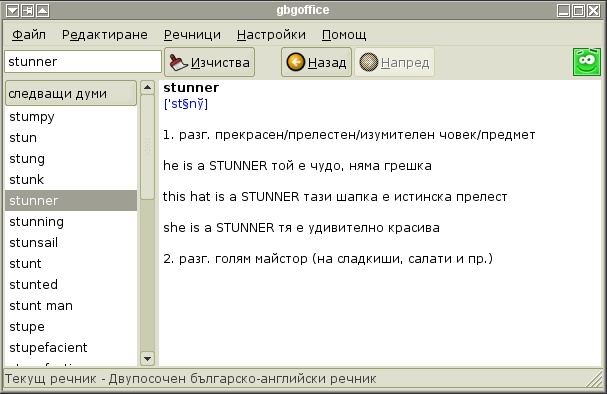
\includegraphics[width=90mm, height=70mm]{images/gbgoffice.jpg}
    \end{figure}

    gbgoffice има версия само за GNU/Linux и FreeBSD, програмата за
    съжаление вече не се поддържа от оригиналния автор, но пък за
    щастие е свободен софтуер и всеки, който има желание може да
    продължи от там, до където той е стигнал.

    gbgoffice не предлага нищо повече от едно речниково приложение - с
    оглед на богатия набор от възможности на Spellbook сравнение между
    двете не би било честно. Единственото предимство на gbgoffice, е
    че като native приложение, написано на C++ консумира много
    по-малко ресурси и работи малко по-бързо. Желаещите да използват
    Spellbook ще трябва да си инсталират Java 6 виртуална машина.
\end{itemize}
\subsection{Конкурентни уеб системи}

\begin{itemize}
  \item \textbf{SA Dictionary}

    SA Dictionary има и уеб версия на адрес http://sa.dir.bg - за
    съжаление тя е още по-постна и от десктоп версията и не предлага
    абсолютно нищо друго освен търсене на дума в речниковата база. В
    интерес на истината, ако не беше надписа "`Powered by SA
    Dictionary"' в долният ляв ъгъл на екрата едва ли някой би
    предположил, че двата проекта имат нещо общо.

  \item \textbf{http://www.rechnik-bg.com/}

    Сайтът http://www.rechnik-bg.com/ предлага някои интересни
    възможности, като например потребителите да добавят думи в
    наличните речници. Сайтът, обаче, не предлага нищо друго освен
    речници и има само уеб версия. Предимство на проекта, е че
    предланите речници са няколко и покриват повечето основни езици.
\end{itemize}

Няма да описвам повече уеб речникови системи, тъй като общо взето
всичките са повече или по-малко същите като гореспоменатите. Колегата
Иван Хантов определено е разработил уеб система за езиково обучение,
която дори и без връзката си с десктоп приложението Spellbook няма
аналог(поне в българското интернет пространство). Когато комбинираме
двете програми - сумата им е уникално и иновативно решение за езиково
обучение, което се надяваме да промени облика на тази част от IT
сегмента в България.

%%% Local Variables: 
%%% mode: latex
%%% TeX-master: "master"
%%% End: 
